\section{リングイメージングチェレンコフ検出器}

\subsection{チェレンコフ放射}
チェレンコフ放射とは、荷電粒子が物質を通過する際に荷電粒子の速度がその物質中の光速を超えると光を発生することである。
またその際の光をチェレンコフ光という。
チェレンコフ光は図のように円錐状に発生する。
この時、チェレンコフ角$\theta_{c}$は物質の屈折率$n$と荷電粒子の速度$\beta$を用いて次のように表せる。

\begin{equation}
  \label{cherenkov_angle}
  \cos \theta_{c} = \frac{1}{n\beta}
\end{equation}

\begin{figure}[htbp]
  \centering
  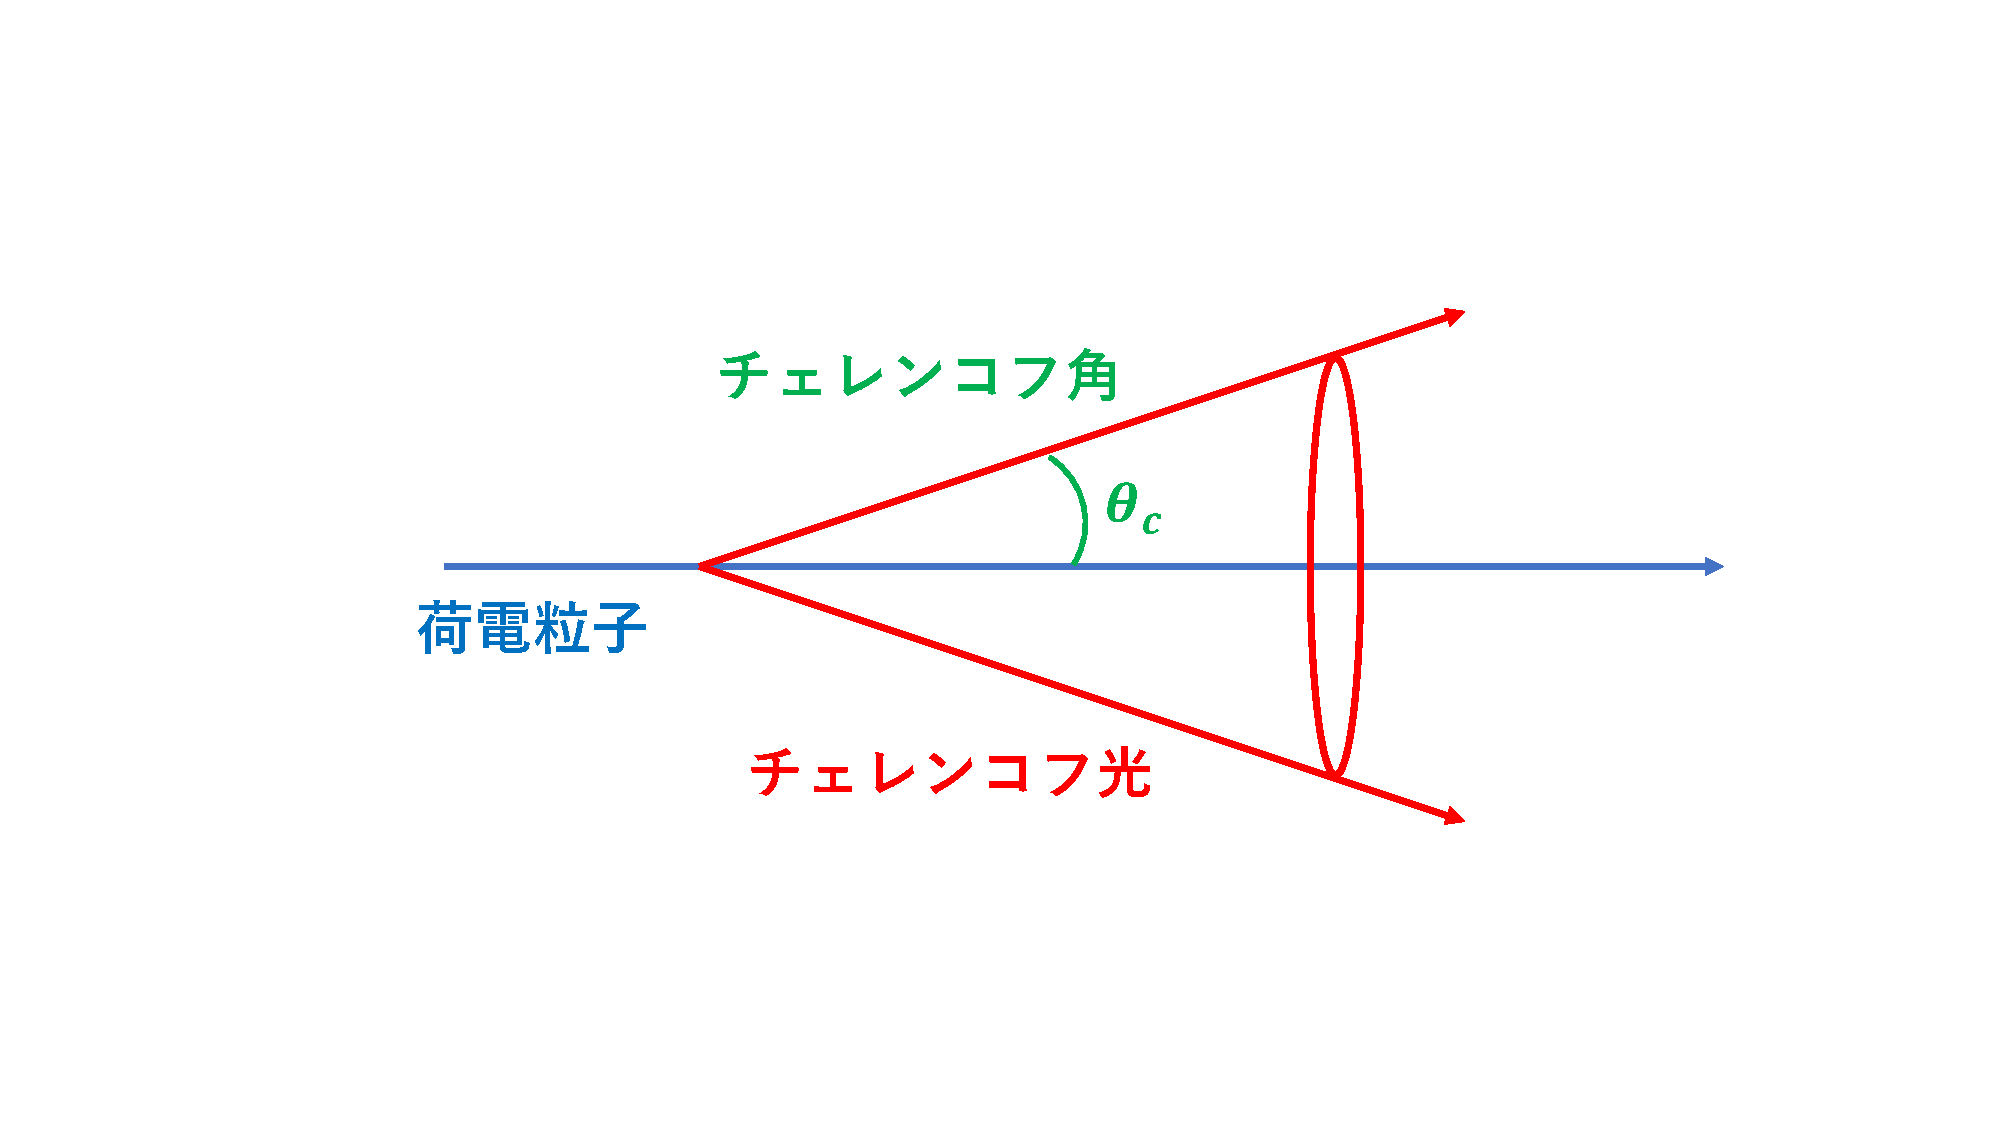
\includegraphics[width=10cm]{images/chapter2/cherenkov.pdf}
  \caption[チェレンコフ放射の模式図]{チェレンコフ放射の模式図。}
  \label{cherenkov}
\end{figure}